%%%%%%%%  Document class  %%%%%%%%%%%%
\documentclass[10pt, letterpaper, fleqn]{article}
% fleqn is for left aligned equations

%%%%%%%%  Packages   %%%%%%%%%%%%%%%%
\usepackage{amsmath,amssymb}
\usepackage{graphicx}
\usepackage{times}
\usepackage{array}
\usepackage{setspace}
\usepackage[backend=bibtex]{biblatex}
\bibliography{C:/Users/Colin/Desktop/R-Projects/INGY/Thesis_files/STCV.bib}

%%%%%%%%  Page Setup %%%%%%%%%%%%%%%%%%
\usepackage[margin= 2cm]{geometry}

%%%%%%%% Document %%%%%%%%%%%%%%%%%%%
\usepackage{Sweave}
\begin{document}
\Sconcordance{concordance:Thesis_doc.tex:Thesis_doc.Rnw:%
7 225 1 1 6 1 2 6 1 1 15 15 1 1 33 5 0 1 2 10 1 1 41 9 1 1 15 23 1 1 26 %
1 3 171 1}

\Sconcordance{concordance:Thesis_doc.tex:Thesis_doc.Rnw:%
7 225 1 1 6 1 2 6 1 1 15 15 1 1 33 5 0 1 2 10 1 1 41 9 1 1 15 23 1 1 26 %
1 3 171 1}


%%%%%%%%  Bibliography Info %%%%%%

\vspace*{5\baselineskip}
\begin{center}
\textbf{\large{Predicting the Growth Response of Small Ponderosa Pine Trees under Varying levels of Overstory Retention, Vegetative Competition and Site Quality}} \\[1pt] 
\vspace*{5\baselineskip}
\text{Colin Kirkmire} \\[1pt]
\vspace*{3\baselineskip}
\text{A thesis submitted to the Graduate Faculty of }\\[1pt]
\text{the University of Montana}\\[1pt]
\text{in partial fullfillment of the}\\[1pt]
\text{requirements for the degree of}\\[1pt]
\text{Master of Science}\\[1pt]
\vspace*{3\baselineskip}
\text{Department of Forest Management}\\[1pt]
\text{College of Forestry and Conservation}\\[1pt]
\text{University of Montana}\\[1pt]
\vspace*{3\baselineskip}
\text{Missoula, Montana}\\[1pt]
\vspace*{1\baselineskip}
\text{{2016}} \\[1pt]
\vspace*{7\baselineskip}
\text{Advised by Dr. David L.R. Affleck and Dr. John Goodburn}\\[1pt]
\vspace*{7\baselineskip}
\end{center}

\newpage
\large 
\begin{center}
\textbf{DEDICATION}\\[1pt]
\end{center}

\newpage
\large 
\begin{center}
\textbf{BIOGRAPHY}\\[1pt]
\end{center}
\normalsize

\newpage
\large 
\begin{center}
\textbf{ACKNOWLEDGEMENTS}\\[1pt]
\end{center}
\normalsize


\newpage
\large 
\begin{center}
\textbf{TABLE OF CONTENTS}\\[1pt]
\end{center}
\normalsize

\newpage
\large 
\begin{center}
\textbf{TABLES}\\[1pt]
\end{center}
\normalsize
\listoftables
\normalsize

\newpage
\large 
\begin{center}
\textbf{FIGURES}\\[1pt]
\end{center}
\normalsize
\listoffigures

\newpage
\large 
\begin{center}
\textbf{LIST OF APPENDICES}\\[1pt]
\end{center}
\normalsize

\newpage
\large 
\begin{center}
\textbf{Introduction}\\[1pt]
\end{center}
\normalsize
\noindent 
\text{This will be the introduction}
\textbf{Objectives}\\[1pt]
\textbf{Ecology of Ponderosa Pine Regeneration}\\[1pt]
This is a test of the citation capabilities of sweave\cite{Riegel1995a}

\newpage
\large 
\begin{center}
\textbf{Methods}\\[1pt]
\end{center}
\normalsize
\textbf{Sampling Strategy}\\[1pt]
\doublespacing
Twenty-nine study sites (termed "installations") were established on a variety of cooperative member ownerships ranging from the eastern slopes of the Cascade Mountains to western Montana. The installations fall within three distinct geographic areas; central Washington, eastern Washington/Idaho and western Montana. \\[4pt]

\begin{figure}[h]
    \centering
    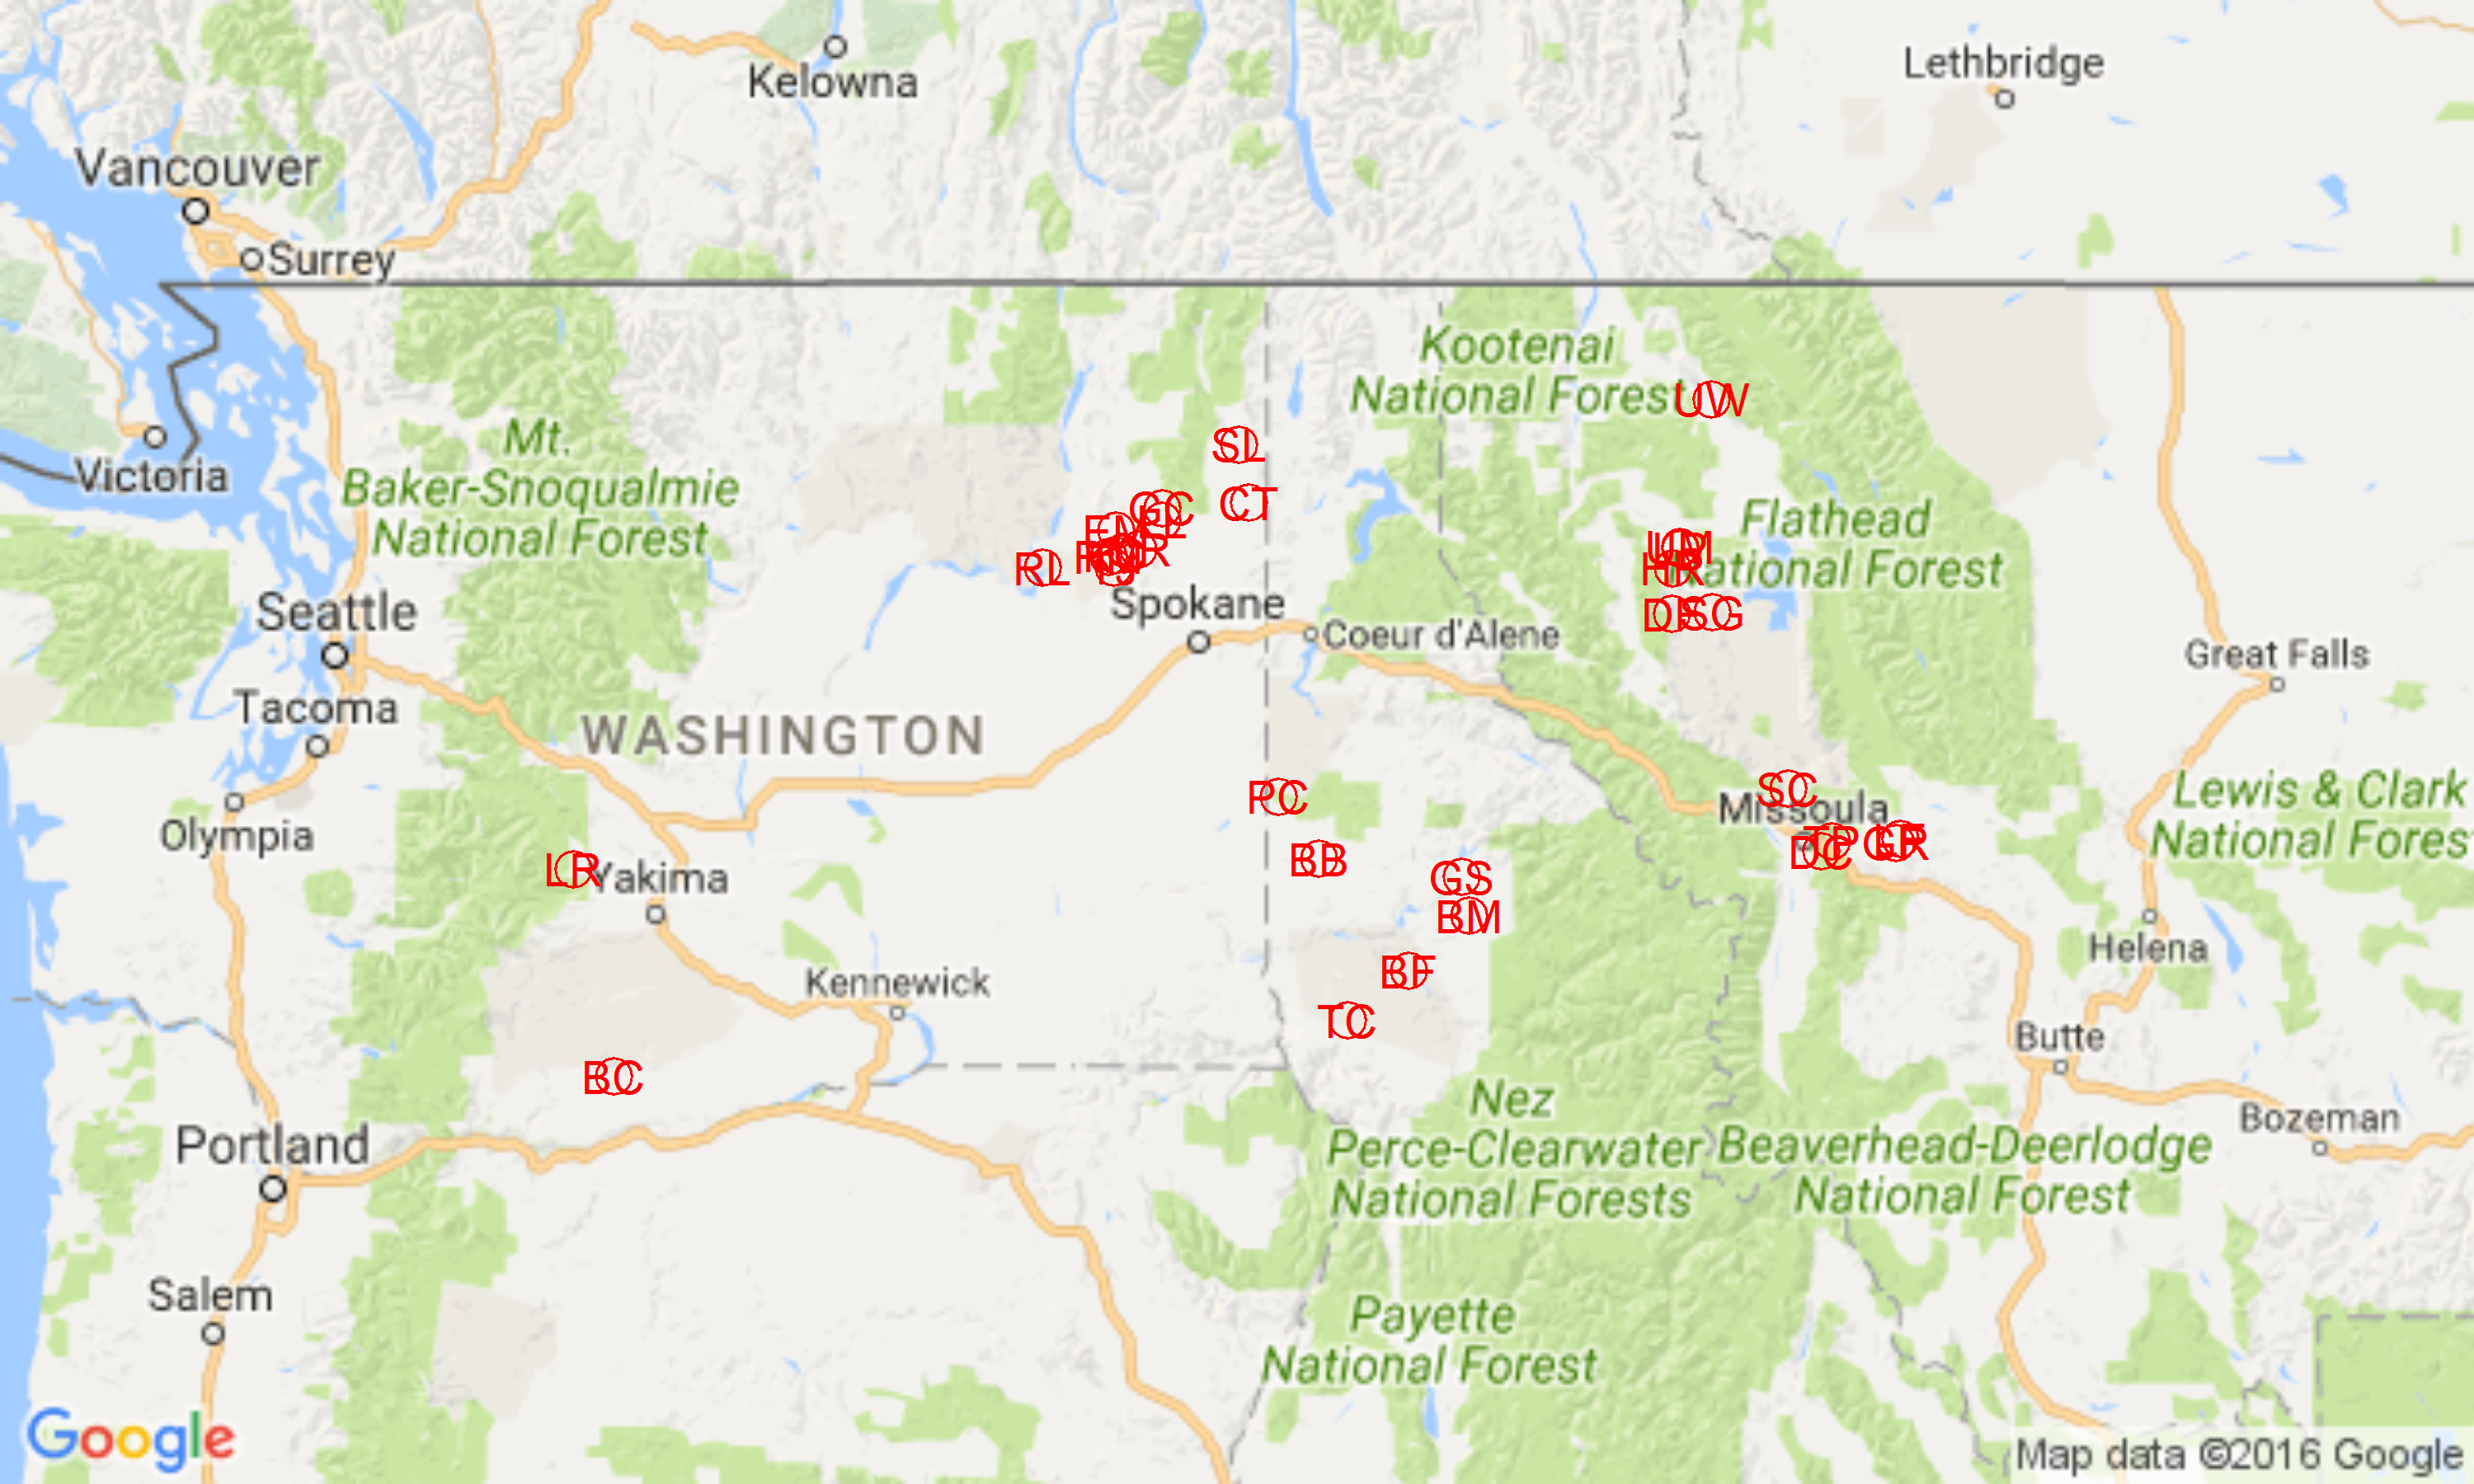
\includegraphics[width=\linewidth]{inst_map.png}
    \caption{a nice plot}
    \label{fig:mesh1}
\end{figure}

Installations were established in stands with various forest cover (e.g., mixed ponderosa pine, Douglas-fir, and grand fir types), with each stand exhibiting relatively homogeneous levels of site quality, overstory tree density, and understory competition.  Installations were located in recently harvested stands that were either clearcut or harvested with one of the aforementioned variable retention harvest systems: shelterwood, seed tree and heavy thinning. \\[2pt]

The temporal initiation of installations varied with most being established in the last years of the 1990s and early 2000s.  Three check plots were also installed to audit the quality of the data collection efforts. Treatments were randomly assigned to seven plots within each installation (Figure 3).  Three plots received multiple applications of regionally effective herbicide.  The remaining four plots are split between the one-time treatment group (just one application of herbicide) and control plots which received no herbicide treatment.\\[2pt]
\noindent 
The primary objective of the different herbicide treatments is to decouple the direct and indirect effects of removing overstory. The removal of the overstory increases available light which is hypothesized to encourage small tree growth as well as non-tree vegetation.  The herbicide treatments allow us to see how small trees grow under reduced overstory without the presence of a corresponding increase in non-tree vegetation.\\[2pt]
\noindent 
Figure 5 shows the temporal scope of the data collection as well as herbicide applications and overstory measurements. An attempt to capture growth at each installation at four year intervals was successful for many installations but in some cases the intervals are somewhat irregular (i.e., 3-5 years in length). The schedule of measurements was based on the twelve-year projection cycles that were used by participating cooperative members.\\[2pt]
\begin{figure}
\begin{center}
\includegraphics{Thesis_doc-001}
\caption{Tis is a caption}
\end{center}
\end{figure}
\noindent 
A point of concern is that some measurements were taken at times that would not have allowed for the herbicide applications to take full effect. That is, several measurements were concurrent with or followed too quickly after the first herbicide application.  This necessitated careful selection of the appropriate measurement years on a per installation basis.  Ultimately, the growth measurements will be put on the same temporal scale of periodic annual increment regardless of whether they were collected on a 3, 4 or 5-year interval. \\[2pt]
\noindent 
Each plot contains a series of nested plots that decrease in area with physiologically smaller vegetation units (Figure 4). Starting with the full extent of the plot, overstory trees (> 10.5 in DBH) were measured on an approximately half acre. Medium trees, with DBH greater than 3.5 in but less than 10.5 in were measured on a smaller nested plot of roughly a quarter acre.
Small trees were measured on six .007 acre plots 60 degrees apart from plot center at a distance of approximately 30 feet.  Small trees are defined as those that have a DBH less than 3.5 in yet are greater than .5 ft in height for shade tolerant species or 1 ft for shade intolerants at the time of initial measurements.\\[2pt]
\noindent 
There were two sampling methods used to measure vegetative competition. The first was transect based where point measurements of vegetation were obtained at one foot intervals along a 40 ft transect.  We also took vegetation measurements in the middle of the small tree plots in the form of both 1m2 and 4m2 grids. These vegetation measurements quantified separately the amounts of forbs, grasses and shrubs to the species level.  This is an example of how the resolution of the data goes beyond the scope of this analysis though will undoubtedly be of use in future research efforts.\\[2pt]
\noindent 
\textbf{Statistical Approach}\\[1pt]
\noindent 
This research seeks to address the question of how to predict the response distribution of small Ponderosa Pine tree height growth increments.  To achieve this ends, a nonparametric statistical regression technique known as quantile regression will be utilized to fit growth curves over select quantiles of the response distribution heights by a set of ecologically and statistically significant predictors. Thus we will be able to predict the heights of the "fastest", "median" and "slowest" growing trees.
This research has widespread applications in the management of Ponderosa Pine stands since the fastest growing trees are
presumably those that progress into the canopy and those that may be retained with preference in the context of a thinning.\\[2pt]
\noindent 
The model is predictive in the sense that it will attempt to predict the .9 quantile height growth increment. For example, the model will not be able to determine whether specific trees will be projected to be above or below the .9 quantile line but rather predict what the .9 quantile height itself is for a given set of predictors. If enough information was known about these trees to predict which would be the fastest growing trees, it would negate the utility of quantile regression.\\[2pt]
\noindent 
The fact that quantile regression attempts to characterize the entire distribution of heights makes it much more difficult to test and validate than an ordinary least squares regression.  The regression estimates at the selected quantile provide predictions for that specific quantile and it is likely that the predictive ability of the model changes at different quantiles.  For example, the model may predict the median better than the upper quantile. \\[2pt]
\noindent 
To evaluate the model, three quantiles will be fitted to represent the range of the response distribution (.90,.50 and .10).  The height increments from the withheld plot data will then be compared to the height of the predicted quantile regression line for its corresponding predictor variables.  For example, if the .90 quantile plane is a good fit, then theoretically 10\% of the height increments will lie above the plane and 90\% below.  The .50 and .10 planes will be evaluated in a similar manner. \\[2pt]
\noindent 
	If it appears that there is some commonality between the tree height increments that are falling below/above the quantile plane...\\[2pt]
\noindent 
Following this evaluation, a random sample of tagged subject trees will be selected to have their height growth increments predicted in the USFS Forest Vegetation Simulator (FVS).  These predicted height increments will then be evaluated as above.  It is not expected that .90 of the predicted tree heights will fall below that .90 quantiles for example. The FVS small tree growth sub-model is based on a least squares regression equation so it is very unlikely that the predicted heights will correspond to the quantile planes.   Rather, this exercise is to illuminate how far from the actual growth response distribution of FVS predictions can be.\\[2pt]
\noindent 
\textbf{Fitting Quantile Regression}\\[1pt]
\noindent 
Only the installations with a greater than 70\% Ponderosa Pine composition at initiation will be included in the model.  Within these installations, the 6th plot will be withheld as training data.  The check plots and installations that have sustained a post-initiation harvest are also excluded from analysis.  \\[2pt]
\noindent 
The "quantreg" package by Roger Koenker (citation) will be used to fit quantile regression planes individually for the specified quantiles (specified as tau values: .90, .50, .10).  This allows for differences in the selected predictor variables between the quantile planes.  \\[2pt]
\noindent 
The variable selection process for each individual quantile will be guided by the ecological framework behind small tree growth.  This means that the predictor variables will be selected from the four previously mentioned categories of ecological factors that affect tree growth. These are overstory measures, understory non-tree vegetation, site productivity and other small tree measures.  The square root of initial height (height at the beginning of measurement period) will also be included as a predictor of height growth increment since it is clear that square root of initial height explains much of the variability in height growth increment and we are interested in the other predictors.\\[2pt]
\noindent 
Variable selection from within these categories is analogous to that of least squares.   Model building will proceed from category to category with the model of lowest p-value being selected as the model carried forward to the next category. This will result in a parsimonious model that is easily understood and supported by our understanding of the factors surrounding small tree growth. \\[2pt]
\noindent 
However, this process alone fails to account for interaction terms between categories which are easy to imagine being important to small tree growth. For example, site productivity may have a different effect with or without understory vegetation.  To account for this, a forward step-wise building of a final model that consists of all four selected variables and all possible combinations of two-way interaction terms will proceed and the model with the lowest AIC selected. Presumably, any real ecological interaction between factors of small tree growth should be visible among the four most significant predictors within each category.\\[2pt]
\noindent 
Selecting a single dimension from each ecological category of small tree competition also has practical advantages.  If a land manager desired to reproduce a similar set of quantile curves for another ecological system or wanted to compare how small tree growth compared to that of the curves produced in this effort, they would need only to collect a singular measure of competition from each of these categories rather than the extensive measurements that the STCV study has undertaken.\\[2pt]

\printbibliography

\end{document}
